\documentclass[pdftex,12pt,letter]{article}
\usepackage[binary-units=true]{siunitx}
\usepackage[margin=0.75in]{geometry}
\usepackage{verbatim}
\usepackage{graphicx}
\usepackage{cite}
\usepackage{color}
\usepackage[pdftex,pdfpagelabels,bookmarks,hyperindex,hyperfigures]{hyperref}
\usepackage{xspace}
\usepackage{amssymb}



\usepackage{tabularx}
\usepackage{url}




\usepackage[firstpage]{draftwatermark}


\bibliographystyle{unsrt}

\newcommand{\fixme}[1]{\textbf{FIXME: #1}}    
\newcommand{\pd}{protoDUNE\xspace}

\title{The protoDUNE-SP experiment and its prompt processing system}
\date{\today}
\author{M.Potekhin for the DUNE Collaboration}

\begin{document}
\SetWatermarkText{DRAFT}
\SetWatermarkLightness{0.9}
\SetWatermarkScale{3}

\maketitle

\begin{abstract}


\noindent The Deep Underground Neutrino Experiment (DUNE) will employ a uniquely large multi-kiloton
Liquid Argon Time Projection Chamber with separate modules utilizing
single and dual-phase Liquid Argon technologies. An experimental 
program (``protoDUNE'')  has been initiated which includes a beam and cosmic ray test of large-scale DUNE prototypes at CERN in 2018.
The volume of data to be collected by the protoDUNE single-phase detector will amount to a few petabytes
and the sustained rate of data sent to mass storage will be in the range of a few hundred megabyte per second.
The protoDUNE experiment requires substantial Data Quality Monitoring capabilities in order to ascertain the
condition of the detector and its various subsystems. To this end, a Prompt Processing system has been deveoped
which is complementary to Online Monitoring and is characterized by a lower bandwidth, scalable CPU resources
and end-to-end latency on the scale of a few minutes. We present the design of the ProtoDUNE Prompt Processing
system, the current status of its development and testing and issues related to its interfaces and deployment.


\end{abstract}

% \tableofcontents
% \pagebreak

\section{Introduction}
The \pd program aims to validate various aspects of the DUNE technology  before proceeding with
the construction of the large-scale principal DUNE detectors at the Sanford Underground Research Facility \cite{cdrVol1, cdrVol4}.
It  is designed to make a series of measurements of the interactions of charged particles in the Liquid Argon medium.  These
measurements will be performed with a dedicated test beam  at the CERN SPS accelerator complex and will also include
a large number of cosmic ray triggers. The program includes two separate
large LArTPC prototypes, one based on a ``single-phase'' (liquid) technology and
one based on a ``dual-phase'' (liquid/gaseous) TPC readout technology.
Both detectors will be placed in an extension of the CERN North Area Experimental Hall.
The general layout of the experimental area is shown in Fig.\,\ref{fig:np02np04}.
Located in this  area will be enclosures which will house
the elements of the local computing infrastructure (including Data Acquisition).
These enclosures are shown schematically as yellow blocks in the
upper-right portion of Fig.\,\ref{fig:np02np04}, and they will have
a dedicated 20 Gb/s
network connection over optical fiber to the CERN central storage
facilities located in the West Area campus of CERN.  

In the following we shall focus on the Single-Phase prototype which will be referred to as ``protoDUNE-SP''.



%%%%%%%%%%%%%%%%%%%%%%%%
\begin{figure}[tb]
\centering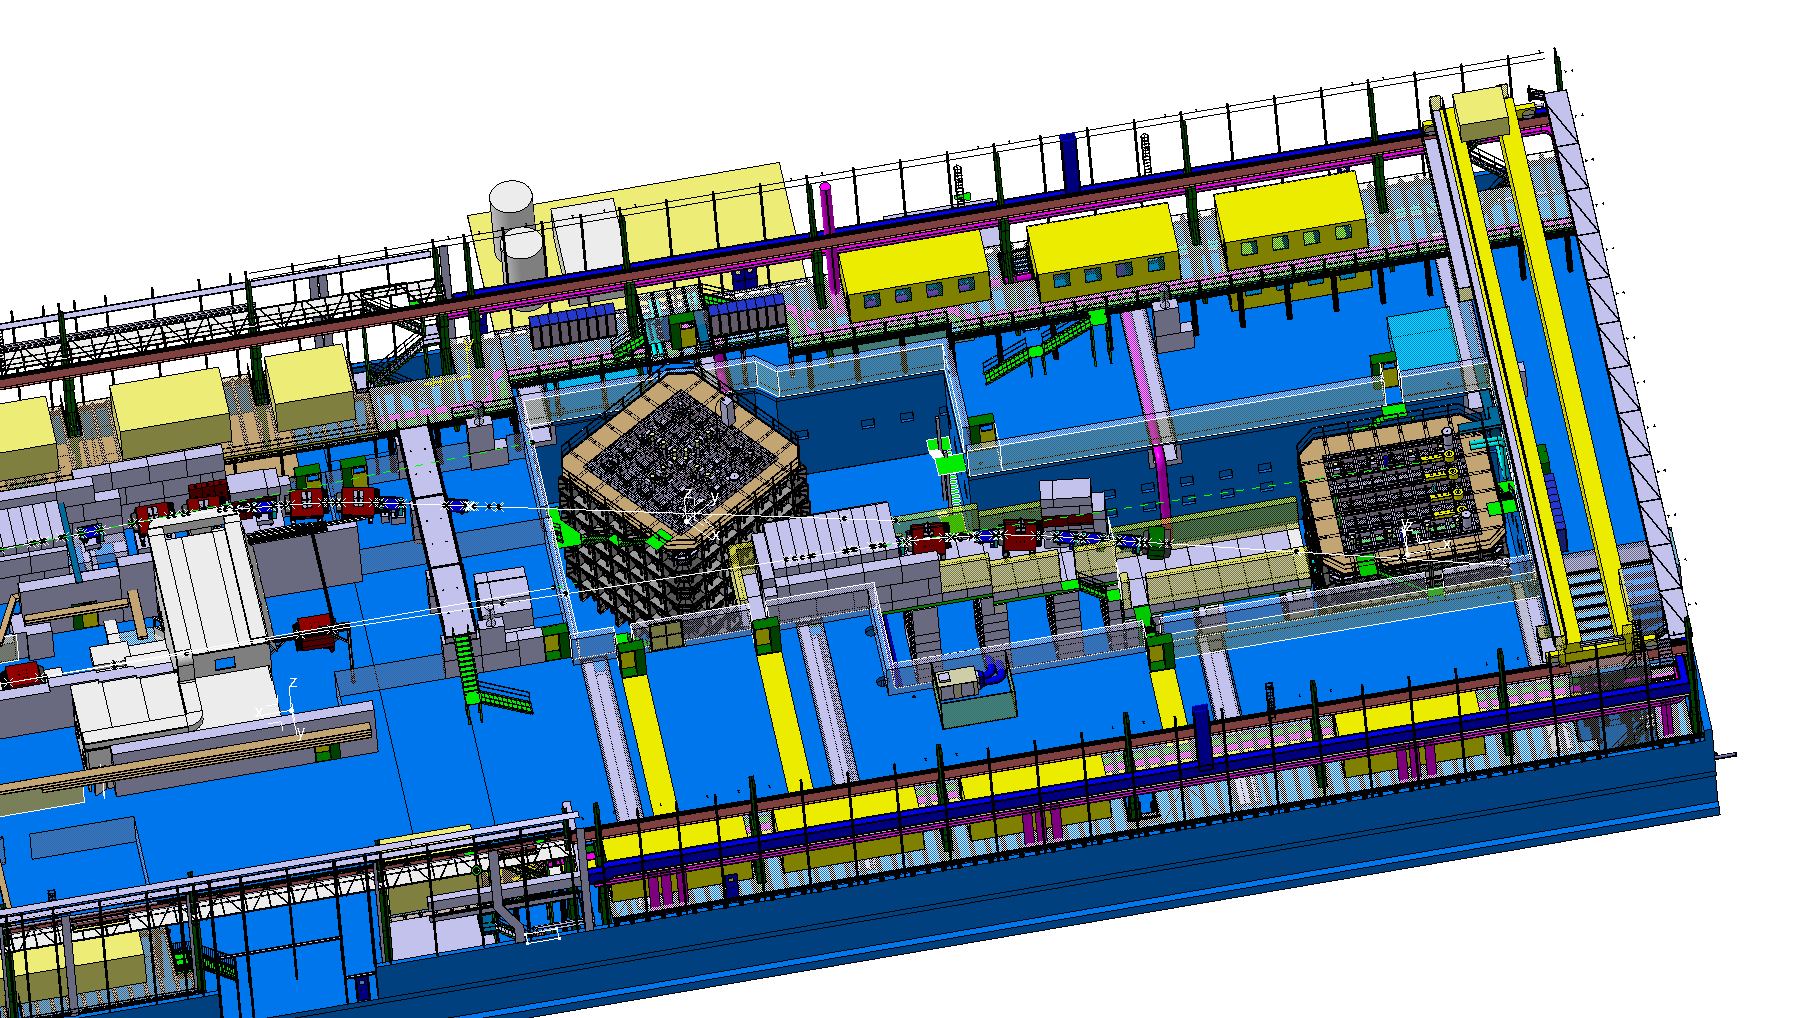
\includegraphics[width=0.8\textwidth]{np02np04.png}
\caption{\label{fig:np02np04}Diagram of the layout of the CERN north area with
  staging of the protoDUNE dual phase detector (center) and single
  phase detector (right).}
\end{figure}
%%%%%%%%%%%%%%%%%%%%%%%%

\section{LArTPC as a Data Source}
\label{sec:np04_data_rate}
DUNE/\pd LArTPC design has a fine spatial resolution due to the high
channel count and spatial granularity, wire pitch and geometry, of the readout
planes.  The readout design also takes advantage the relatively slow
drift velocity of ions in the Argon and the 2\,MHz digitization clock
to achieve similarly fine spatial and temporal resolution along the
drift axis of the detector. The readout window is  set to 5\,ms 
which is driven by the electron drift time across
the active volume (which is slightly less).  These characteristics are typical of
similar modern TPC detectors.

In the absence of zero suppression these factors do however
result in a large data volume that needs to be read out and
processed for a single readout.
%single considerable amount of data collected per single event readout (trigger).
A DUNE/\pd readout event may be compared to sequential stack of a thousand of digital
images of the signals collected from the electrodes. 
The instantaneous triggered data rate and the data rates averaged over
the beam's spill and duty factors are expected to be primarily limited
by the network bandwidth available within the DAQ infrastructure and
the I/O bandwidth available for recording the data.  Lossless data
reduction/compression (e.g. Huffman encoding)
techniques are applied to the data within the DAQ readout chain and
are projected to result in a factor of 4x reduction to the raw data.
Based on these projections, the NP04 experiment is expected to accumulate 2.5~PB of physics beam
data during 3 months of running.  The total data volume accumulated by
the experiment is expected to be larger when data from
detector commissioning prior to the beam run, and cosmic ray data from
after the beam running are included.   These rates are detailed in Table.\,\ref{table:np04_data_rate}.

% \section{The NP04 Data Characteristics}
% \label{sec:np04_data_rate}
% The following nominal parameters define the expected data rates and volume in NP04:
% \begin{itemize}
% \item TPC channel count: 15,360
% \item Digitization frequency: 2MHz
% \item Readout window: 5\,ms
% \item Trigger rate: 100\,Hz
% \item SPS spill time: 4.8\,s
% \item SPS cycle: 16.8\,s
% \item Compression: $\times$4
% \end{itemize}
% \noindent This results in the following nominal data characteristics:
% \begin{itemize}
% \item Instantaneous rate (in DAQ): 11.5\,GB/s
% \item Average rate (including ingestion into mass storage): 3.3\,GB/s
% \item Total data to be captured: 6\,PB
% \item Buffer to store 3 days worth of data: 850\,TB
% \end{itemize}

\begin{table}
\begin{center}
\caption[GPS Detector Locations]{\label{table:np04_data_rate}
  Detector, beam, DAQ and data rate parameters for the single phase
  \pd experiment (NP04).}
\ \\
\begin{tabularx}{0.75\textwidth}{ X  >{\setlength{\hsize}{0.8\hsize}}r}
\hline
Detector Parameter & Target \\
\hline
TPC channel count & 15,360 \\
Digitization frequency & 2\,MHz \\
Readout window & 5\,ms \\
SPS spill time& 4.8\,s\\
SPS cycle& 22.5\,s\\
Trigger rate (target minimum/maximum) & 25--100\,Hz \\
Single readout size (per trigger) & 230.4\,MB \\
Target compression factor& $\times$4 \\
Instantaneous data rate (in-spill) & 1440\,MB/s \\
Average data rate & 576\,MB/s \\
Total data recorded (beam + cosmic) & 2.5\,PB\\
Buffer to store 3 days worth of data & 300\,TB\\
\hline
\end{tabularx}
\end{center}
\end{table}





\clearpage

\section*{References}
\begin{thebibliography}{9}

\bibitem{cdrVol1}
R Acciarri et al.
``Long-Baseline Neutrino Facility (LBNF) and Deep Underground Neutrino Experiment (DUNE) Conceptual Design Report Volume 1: The LBNF and DUNE Projects''.\\ e-Print: arXiv:\textbf{1601.05471}
 %DUNE CDR Vol 1 -- The LBNF and DUNE Projects.~e-Print: arXiv:1601.05471
%\url{http://arxiv.org/abs/1601.05471}

\bibitem{cdrVol4}
R Acciarri et al.
``Long-Baseline Neutrino Facility (LBNF) and Deep Underground Neutrino Experiment (DUNE) Conceptual Design Report, Volume 4 The DUNE Detectors at LBNF''.\\~e-Print: arXiv:\textbf{1601.02984}
%\url{http://arxiv.org/abs/1601.02984}

%\bibitem{np04} 
% Yearly report on ProtoDUNE Single Phase NP04 (2016), \textit{CERN-SPSC-2016-018}
%\url{https://cds.cern.ch/record/2144868}

\bibitem{xrootd}
L Bauerdick et al. ``Using Xrootd to Federate Regional Storage.'' \textit{J. Phys.: Conf. Series.} Vol.\textbf{396}. IOP Publishing, 2012.
%{XRootD software framework:}~\url{http://www.xrootd.org}

%\bibitem{cenf}
%{CERN Neutrino Platform}\\
%\url{http://home.cern/about/experiments/cern-neutrino-platform}


\bibitem{castoreos}
 L Mascetti et al. ``Disk storage at CERN.'' \textit{J. Phys.: Conf. Series.} Vol.\textbf{664}. IOP Publishing, 2015.
%{CASTOR -- CERN Advanced STORage manager}:~
%\url{http://castor.web.cern.ch/}

%\bibitem{eos}
%{The CERN Exabyte Scale Storage}\\
%\url{http://information-technology.web.cern.ch/services/eos-service}


\bibitem{sam}
R A Illingworth ``A data handling system for modern and future Fermilab experiments.''  \textit{J. Phys.: Conf. Series.} Vol.\textbf{513}. IOP Publishing, 2014.

%{A data handling system for modern and future Fermilab experiments}\\
%\url{http://iopscience.iop.org/1742-6596/513/3/032045}

\bibitem{fts}
Norman A 2014 \textit{The Fermilab File Transfer System}.~e-Print: FNAL CD-DocDB-5412
%%\url{http://cd-docdb.fnal.gov/cgi-%bin/RetrieveFile?docid=5412&filename=datamanagement-
%%changeprocedures.pdf&version=1}

\bibitem{nova}
R Plunkett et al.  ``Status of the NOvA Experiment.''  \textit{J. Phys.: Conf. Series.} Vol.\textbf{120}. IOP Publishing, 2008.


% NOvA Neutrino Experiment:~
% \url{https://www-nova.fnal.gov/}

\bibitem{uboone}
B Jones et al.  ``The Status of the MicroBooNE Experiment.''  \textit{J. Phys.: Conf. Series.} Vol.\textbf{408}. IOP Publishing, 2013.

%The MicroBooNE Experiment:~
% \url{http://www-microboone.fnal.gov/}

\bibitem{dcache}
A Millar et al.  ``dCache, agile adoption of storage technology.''  \textit{J. Phys.: Conf. Series.} Vol.\textbf{396}. IOP Publishing, 2012.
% {dCache, a distributed storage solution:}~
% \url{https://www.dcache.org/}

%\bibitem{larsoft}
%{LArSoft Collaboration}:~
%\url{http://larsoft.org//}

\end{thebibliography}



\end{document}

%%% Local Variables:
%%% mode: latex
%%% TeX-master: t
%%% End:
\grid
